
\documentclass[draft2.tex]{subfiles} 
\begin{document} 

\section{Acknowledgements} 
\label{sec:acknowledgements} 

% fig 18 
\begin{figure*} 
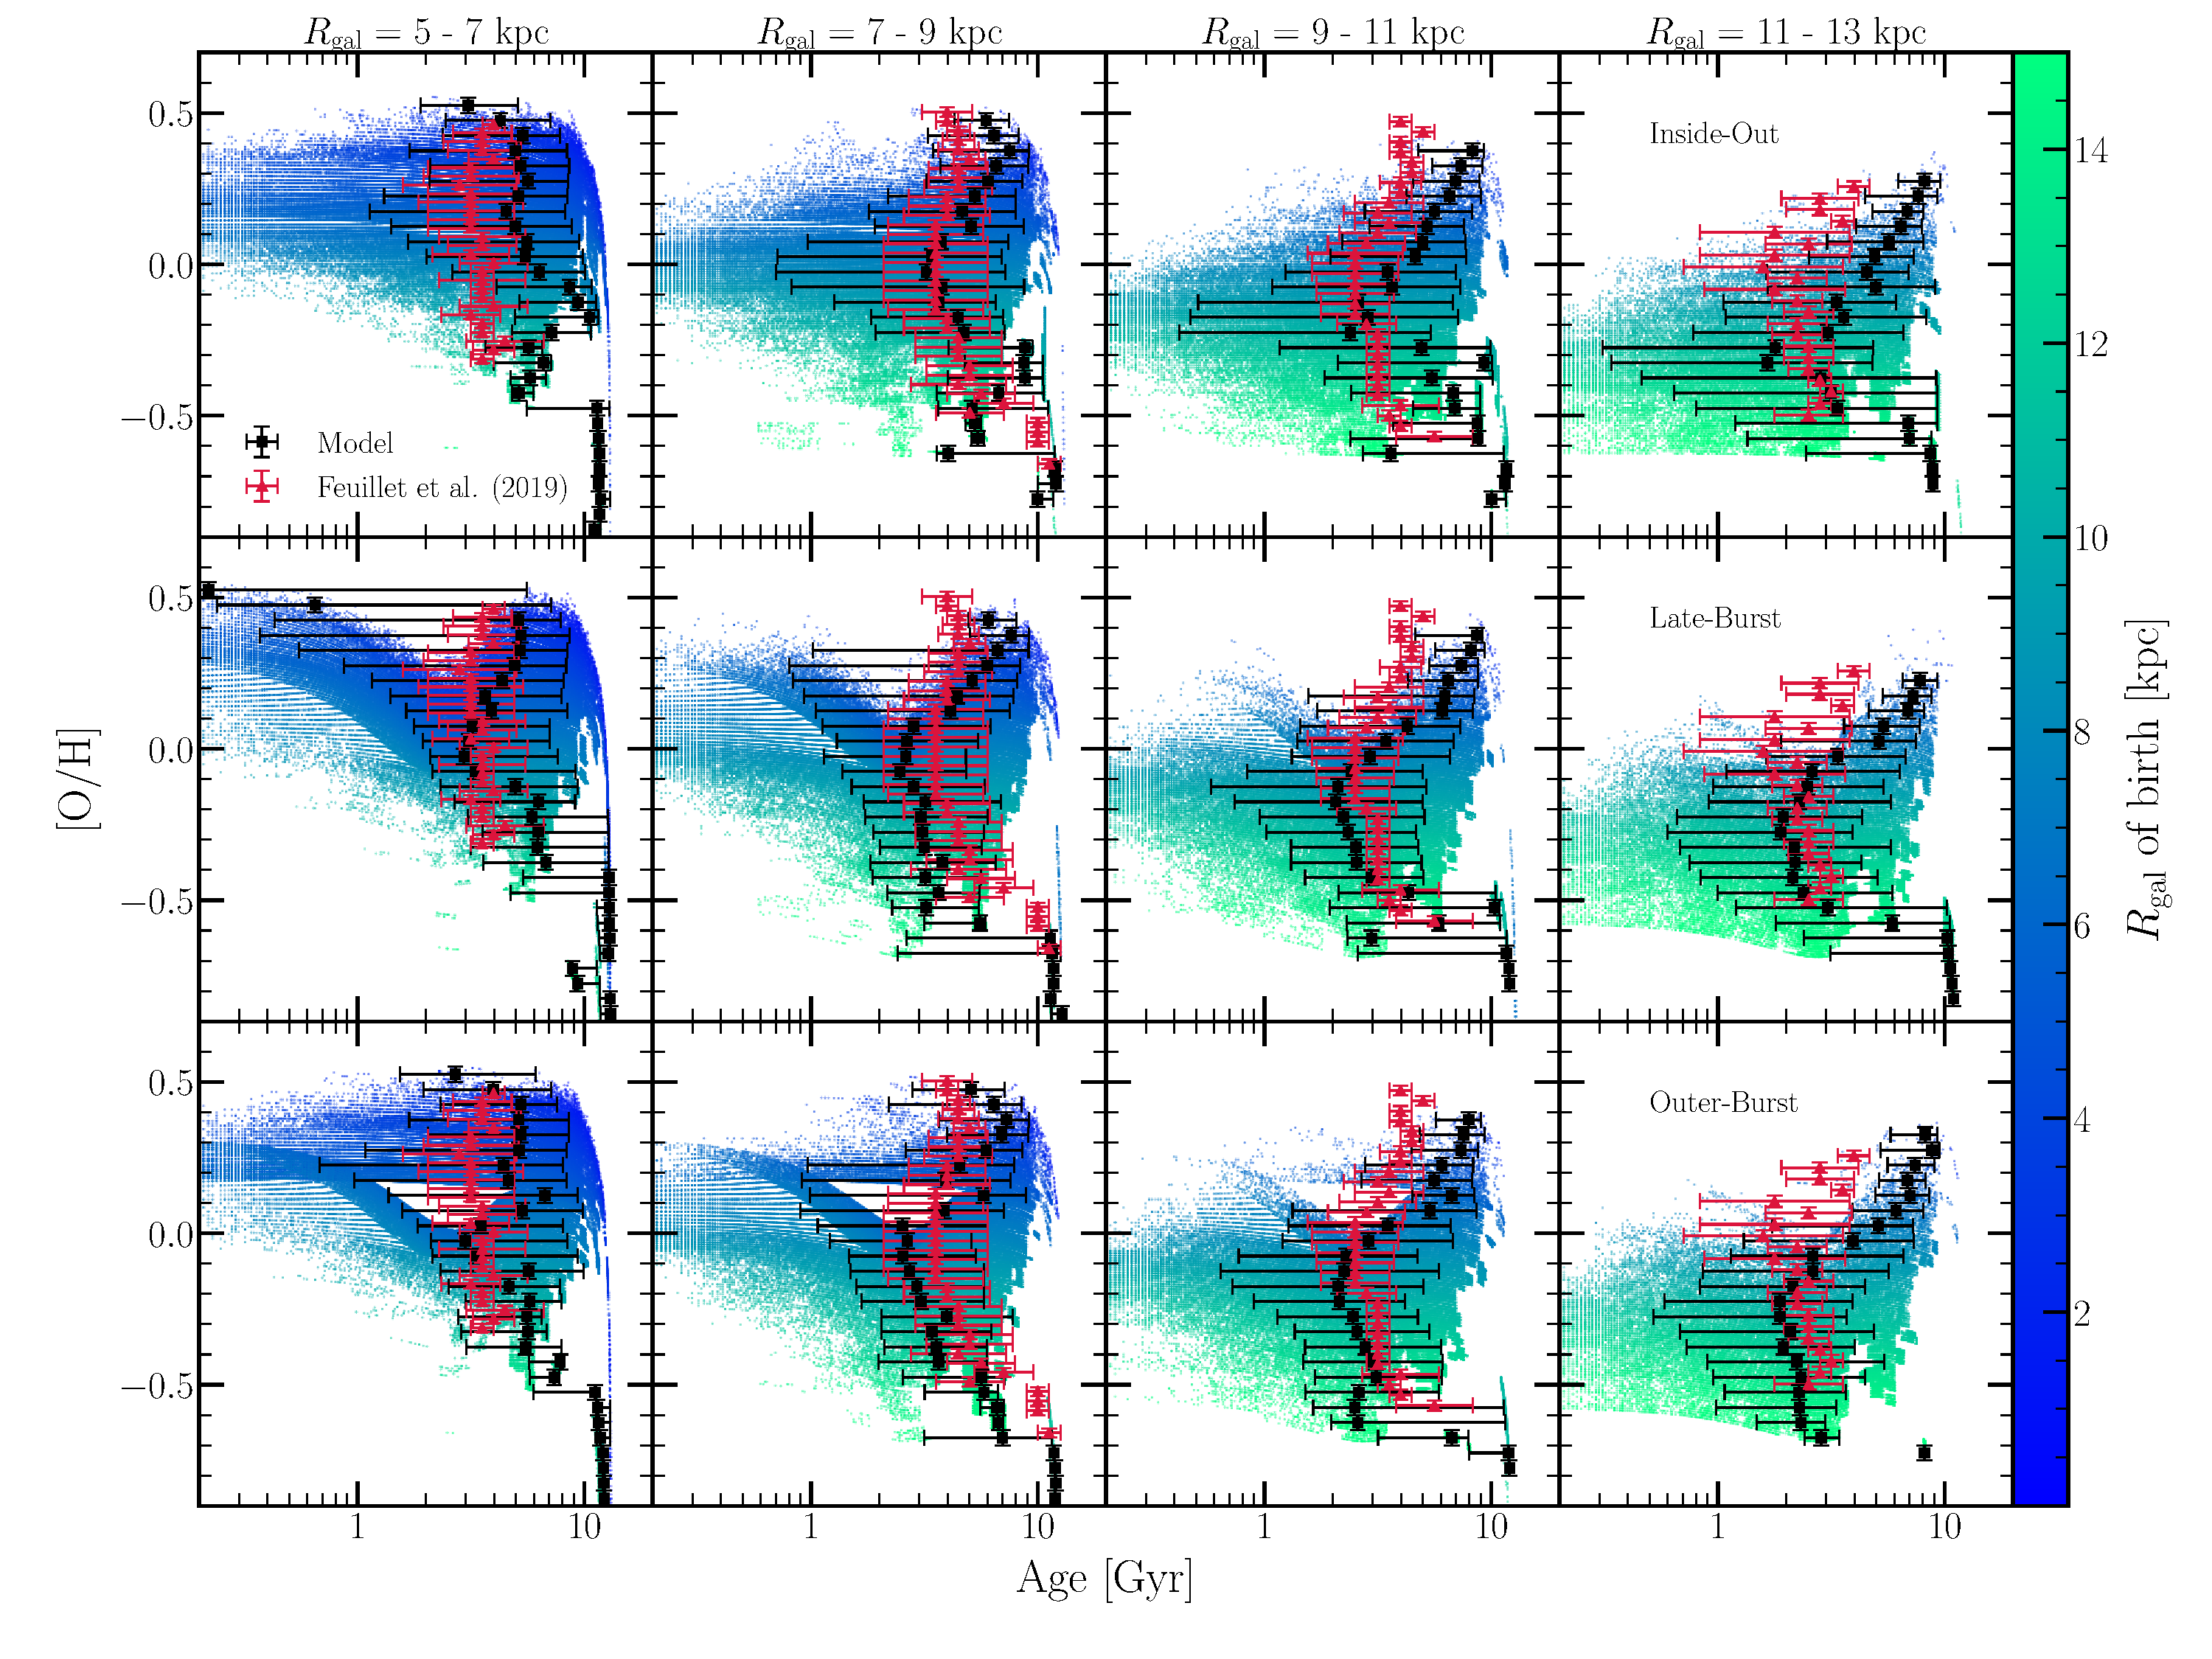
\includegraphics[scale = 0.32]{age_oh_comparison.pdf} 
\caption{The same as Fig.~\ref{fig:amr_insideout_vs_lateburst_fe}, but for 
\oh, and with an additional comparison to the outer-burst model in the 
bottom row.} 
\label{fig:age_oh_comparison} 
\end{figure*} 

We acknowledge valuable discussion with Jennifer Johnson, Adam Leroy, Grace 
Olivier, Amy Sardone, Jiayi Sun, Todd Thompson, and other members of the Ohio 
State Astronomy Gas, Galaxies, and Feedback group, as well as various 
participants of the SDSS Gotham 2020 virtual collaboration meeting and the 
virtual 236th meeting of the American Astronomical Society. 
We thank Diane Feuillet for providing the results of~\citet{Feuillet2019} in 
digital form. 
This work was supported in part by National Science Foundation grant 
AST-1909841. 
D.H.W. is grateful for the hospitality of the Institute for Advanced Study and 
the support of the W.M. Keck Foundation and the Hendricks Foundation. 
F.V. acknowledges the support of a Fellowship from the Center for Cosmology and 
AstroParticle Physics at the Ohio State University. 
\par 
In this paper we have made use of data from SDSS-IV APOGEE-2 DR16. 
Funding for the Sloan Digital Sky 
Survey IV has been provided by the 
Alfred P. Sloan Foundation, the U.S. 
Department of Energy Office of 
Science, and the Participating 
Institutions. 
\par 
SDSS-IV acknowledges support and 
resources from the Center for High 
Performance Computing  at the 
University of Utah. The SDSS 
website is~\url{www.sdss.org}.
\par 
SDSS-IV is managed by the 
Astrophysical Research Consortium 
for the Participating Institutions 
of the SDSS Collaboration including 
the Brazilian Participation Group, 
the Carnegie Institution for Science, 
Carnegie Mellon University, Center for 
Astrophysics | Harvard \& 
Smithsonian, the Chilean Participation 
Group, the French Participation Group, 
Instituto de Astrof\'isica de 
Canarias, The Johns Hopkins 
University, Kavli Institute for the 
Physics and Mathematics of the 
Universe (IPMU) / University of 
Tokyo, the Korean Participation Group, 
Lawrence Berkeley National Laboratory, 
Leibniz Institut f\"ur Astrophysik 
Potsdam (AIP),  Max-Planck-Institut 
f\"ur Astronomie (MPIA Heidelberg), 
Max-Planck-Institut f\"ur 
Astrophysik (MPA Garching), 
Max-Planck-Institut f\"ur 
Extraterrestrische Physik (MPE), 
National Astronomical Observatories of 
China, New Mexico State University, 
New York University, University of 
Notre Dame, Observat\'ario 
Nacional / MCTI, The Ohio State 
University, Pennsylvania State 
University, Shanghai 
Astronomical Observatory, United 
Kingdom Participation Group, 
Universidad Nacional Aut\'onoma 
de M\'exico, University of Arizona, 
University of Colorado Boulder, 
University of Oxford, University of 
Portsmouth, University of Utah, 
University of Virginia, University 
of Washington, University of 
Wisconsin, Vanderbilt University, 
and Yale University.

\textit{Software}: Matplotlib~\citep{Matplotlib}; Astropy~\citep{Astropy2013, 
Astropy2018}; NumPy~\citep{NumPy}. 

\end{document} 
